\chapter{Path planning theory}
An autonomous system must be able to create a plan on how the system should move around in the surrounding environment in a feasible way. A minimum requirement for a path is that it is connected. The connection level can be described by the paths smoothness. Parametric continuity is denoted $C^n$ were n is the degree of smoothness. The order of n implies that the n first parametric derivatives match at a common point for two subsequent paths \citep{barsky1989geometric}. Geometric continuity is a relaxed from of parametric continuity in witch discontinuousness in speed is allowed. A table of geometric and parametric continuity lists the requirement for each smoothness level \ref{TB:SmoothnessDescriptions}, which is based definitions presented in \citep{barsky1989geometric}.
Geometric continuity is sufficient for a path following system, which is the main focus of this thesis. Geometric continuity is denoted as $G^n$ were n is the order of continuity.

\begin{table}[H]
\begin{center}
\begin{tabular}{| l | | l |}
\hline
\textbf{Geometrical smoothness level} & \textbf{Description} \\ \hline
$G^0$ & All subpaths are connected \\ \hline
$G^1$ & The path-tangential angle is continuous \\ \hline
$G^2$ & The center of curvature is continuous \\ \hline
\textbf{Parametric smoothness level} & \textbf{Description} \\ \hline
$C^0$ & All subpaths are connected \\ \hline
$C^1$ & The velocity is continuous \\ \hline
$C^2$ & The acceleration is continuous \\ \hline
\end{tabular}
\end{center}
\caption{Smoothness definitions}
\label{TB:SmoothnessDescriptions}
\end{table} 

The definition used for path in this thesis is equation 1.2 in \citep{tsourdos2010cooperative} which state:
\begin{equation}
P_s(x_s,y_s,z_s,\theta_s,\psi_s) \xrightarrow{r(q)} P_f(x_f,y_f,z_f,\theta_f,\psi_f)
\end{equation}
where the subscripts $s$ and $f$ denotes the start pose and finish pose respectfully with $r(q)$ as the path.

\section{Straight lines}
The simplest form on path is a straight line between $P_s$ and $p_f$. The straight line is given as 
\begin{subequations}
\begin{align}
& x(s) = a_xs + b_x \\
& y(s) = a_ys + b_y 
\end{align}
\end{subequations}
with $ s \in [0,1] $, where $s$ has not necessary a physical meaning. Then the parametrisation of the straight line is:
\begin{subequations}
\begin{align}
& x(0) = b_x \rightarrow b_x = x_s \\
& x(1) = x_f = a_x + b_x \rightarrow a_x = x_f - b_x \\
& y(0) = b_y \rightarrow b_y = y_s \\
& y(1) = y_f = a_y + b_y \rightarrow a_y = y_f - b_y \\
\end{align}
\end{subequations}
The tangential vector for a straight line is given as:
\begin{equation}
\psi (s) = \atan2(a_x,a_y)
\end{equation}
A path constructed by straight lines is $G^0$, however since the tangential vector is discontinuous between two line segments with different heading it's not $G^1$. The disadvantage with a path which is $G^0$ is that large discontinuity between two tangential vectors will cause problem for a control system. 
\begin{figure}[H]
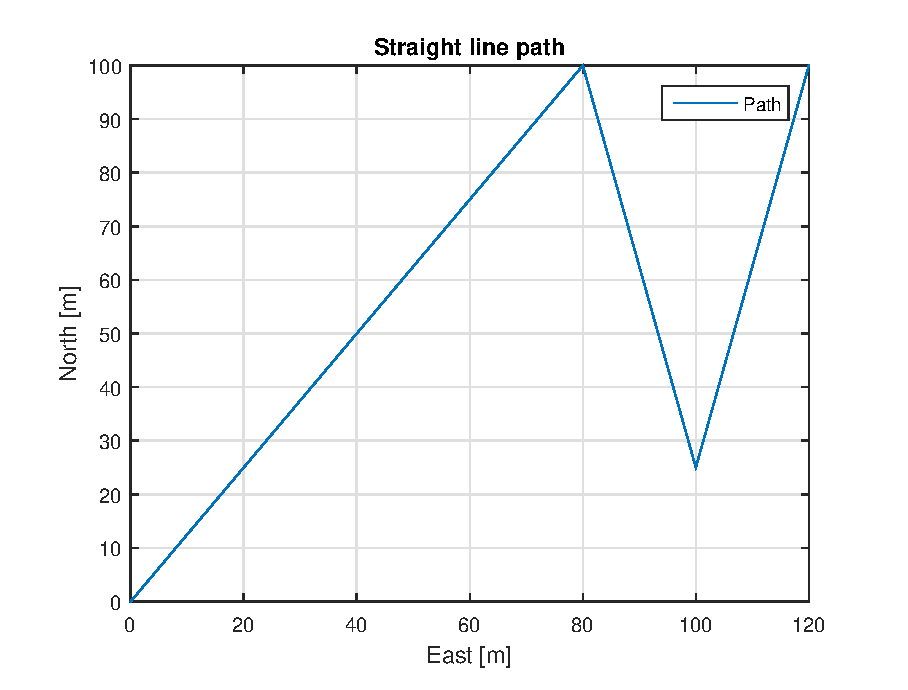
\includegraphics[width=0.7\textwidth]{figs/TheoryPlot/StraightLine.eps}
\caption{Straight line path}
\end{figure}
The simplest for of creating a path is a straight line between two way-points. The advantage with a straight line is that it's easy for a guidance system to follow the line, however it will experience a jump in reference when transitioning to another straight line due to discontinuous tangential vector.
\section{Dubins path}\label{S:DubinsPath}
An alternative to a straight line path is a path constructed by straight lines and circle. Such a path is Dubins path\citep{dubins1957curves}, which showed that the shortest possible path for a particle that moved with unit speed with maximum curvature would consist of two circles and a straight line. The path consist of two arcs and a straight line. The straight line is tangential to both arcs. A disadvantage with Dubins path is that the curvature is discontinues, which gives a path from $P_s$ to $P_f$ with smoothness level of $G^1$.

A Dubins path that is constructed where the final orientation is fixed has four different ways to be constructed, which is determined by the rotation directions. The four types of Dubins path that is used in this thesis is given in table \ref{Tb:DubinsTurningDirection}.
\begin{table}[H]
\centering
\begin{adjustbox}{max width=\textwidth}
\begin{tabular}{ | l |}
\hline
Right to Right \\
Right to left \\
Left to Right \\
Left to left \\ \hline
\end{tabular}
\end{adjustbox}
\caption{Turning direction for Dubins path with fixed final orientation}
\label{Tb:DubinsTurningDirection}
\end{table}
The equations that is used to construct the path is found in \citep{tsourdos2010cooperative} section 2.2.1, with a constructed path shown in figure \ref{Fig:DubinsPath}. 
\begin{figure}\label{Fig:DubinsPath}
\def\svgwidth{\textwidth} % Defining the width since Inkscape hasn't done this yet in the .pdf_tex file
\input{InkFig/DubinsPath.pdf_tex}
\caption{Dubins path}
\end{figure}
The first step if to determine the start and final turning circle center. The center is found with the equations:
\begin{subequations}
\begin{align}
& X_{cs} = X_s - R_s\cos(\psi_s \pm \frac{\pi}{2}) \\
& Y_{cs} = Y_s - R_s\sin(\psi_s \pm \frac{\pi}{2}) \\
& X_{cf} = X_f - R_f\cos(\psi_f \pm \frac{\pi}{2}) \\
& Y_{cf} = Y_f - R_f\sin(\psi_f \pm \frac{\pi}{2})
\end{align}
\end{subequations}
where $R_s$ and $R_f$ is the radius of the start and final turning circle respectfully, with $\psi_s$ and $\psi_f$ the start and final heading. The centres for the start and final turning circle is defined as:

\begin{align}
& O_{cs} =
\begin{bmatrix}
X_{cs} \\
Y_{cs}
\end{bmatrix} \\
& O_{cf} =
\begin{bmatrix}
X_{cf} \\
Y_{cf}
\end{bmatrix}
\end{align}
Continuing the centres $O_{cs}$ and $O_{cf}$ is connected with a centreline $c$, where the length is:
\begin{equation}
|c| = \sqrt{(X_{cs}-X_{cf})^2+(Y_{cs}-Y_{cf})^2}
\end{equation}
The arc exit and entry point for the start and final circle is calculated by first applying the equations:
\begin{subequations}
\begin{align}
& \alpha = \arcsin\big(\frac{R_f-R_s}{|c|}\big) \\
& \beta = \arctan\big(\frac{X_{cf}-X_{cs}}{X_{cf}-X_{cs}}\big)
\end{align}
\end{subequations}
where $\alpha$ is the angle between the length of the center line between the two circles, and the length of the line from the start circle to the exit tangent point. $\beta$ is the angle of the center line. The exit and entry tangent point is found with the use of table \ref{Tb:ExitEntyrTangent}.
\begin{table}[H]
\begin{center}
\begin{tabular}{ | l | | l |}
\hline
& \textbf{Turn angle} \\ \hline
$\phi_{right}$ & $\alpha + \beta + \frac{\pi}{2}$ \\
$\phi_{left}$ & $\beta - \alpha + \frac{3\pi}{2}$ \\ \hline
\end{tabular}
\end{center}
\label{Tb:ExitEntyrTangent}
\end{table}
With the angle of the exit and entry tangent point the point is given as:
\begin{subequations}
\begin{align}
& x_{P_\chi} = x_{cs} + R_s\cos(\phi) \\
& y_{P_\chi} = x_{cs} + R_s\sin(\phi) \\
& x_{P_N} = x_{cf} + R_f\cos(\phi) \\
& y_{P_N} = x_{cf} + R_f\sin(\phi)
\end{align}
\end{subequations}
%\begin{figure}[H]
%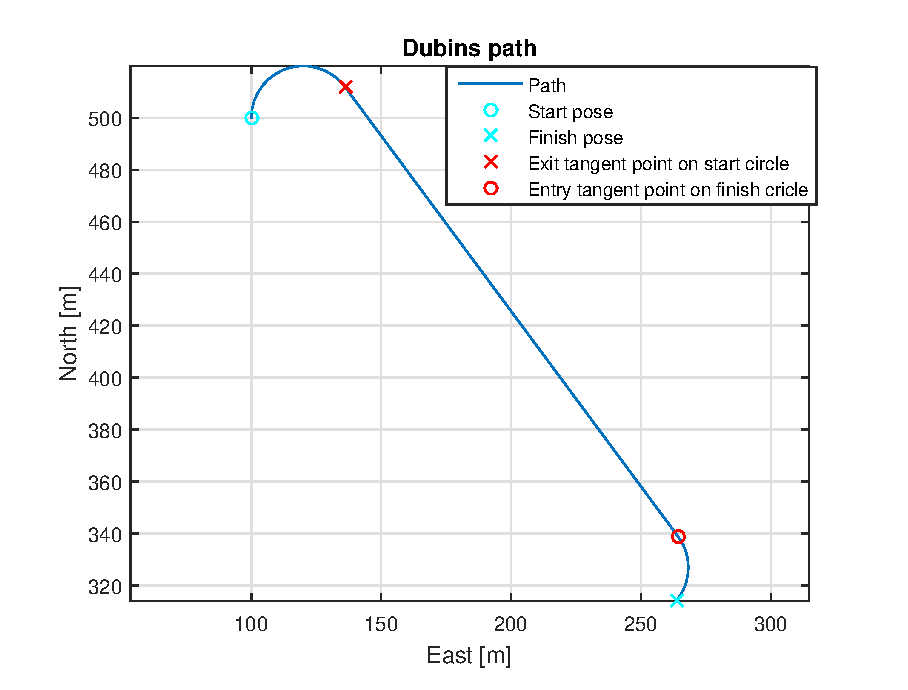
\includegraphics[width=0.7\textwidth]{figs/TheoryPlot/DubinsPath.eps}
%\end{figure}
The length of the path is calculated in three parts. The first the is the arc length from the start pose to the exit tangent point, then the length of the straight line before the arc length from the entry point to the final pose. The length of the path is given as: 
\begin{equation}
d = R_s\phi_s + d_t + R_f\phi_f
\end{equation}
where $d_t = ||P_N-P_{\chi}||_2$, $\phi_s$ and $\phi_f$ is the arc angle for the start and final circle respectfully.